\begin{table*}[t]
\vspace{-0.em}
\centering
\captionsetup{justification=centering}
 \caption{Performance (\emph{Success Rate}) for different PAMDP methods over resource-limited environments. \\ Results are averaged over five random seeds, $\pm$ indicates the standard deviation across seeds, and bold entries denote the best performance.}
 \label{tab:main_result}
\resizebox{1.0\textwidth}{!}{%
\begin{tabular}{c c >{\columncolor{gray!25}}c c c c c c c}
\toprule
 \multicolumn{2}{c}{\textbf{Task/ Scenario}} & \textbf{TART} & \textbf{PADDPG}~\cite{hausknecht2015deep} & \textbf{PDQN}~\cite{xiong2018parametrized} & \textbf{HPPO}~\cite{fan2019hybrid} & \textbf{HyAR}~\cite{li2021hyar} & \textbf{TART w/o $\mathcal{L}_{\text{NCE}}$} & \textbf{TART w/o $\mathcal{L}_{\text{VQ}}$} \\
\midrule
\multirow{2}{*}{Maze Navigation}  & Easy & $\mathbf{97.2\pm 1.3}$ & $88.2\pm 6.9$ & $85.8\pm 6.1$ & $87.2\pm 4.6$ & $94.5\pm 3.2$ & $92.8\pm 3.3$ & $95.4 \pm 1.9$ \\
                             & Medium & $\mathbf{90.8\pm 4.2}$ & $74.2 \pm 6.1$ & $68.8 \pm 6.2$ & $74.6 \pm 9.0$ & $80.6\pm 8.5$ & $89.0\pm 3.5$ & $88.2\pm 5.3$ \\ 
                             & Hard & $\mathbf{72.8\pm 9.9}$ & $38.8 \pm 10.5$ & $38.4\pm 13.5$ & $46.2\pm 6.7$ & $60.4\pm 9.1$ & $69.2\pm 5.7$ & $67.0\pm 3.2$ \\  
\midrule

\multirow{2}{*}{Air-to-Air Combat} & Easy & $\mathbf{94.8\pm 3.1}$ & $79.6\pm 5.6$ & $81.2\pm 5.9$ & $87.8\pm 4.6$ & $86.6\pm 4.8$ & $92.4\pm 5.1$ & $91.8\pm 2.2$ \\ 
                             & Medium & $\mathbf{90.8\pm 4.2}$ & $68.6\pm 5.9$ & $74.2\pm 4.3$ & $76.2\pm 4.5$ & $77.6\pm 6.3$ & $87.0\pm 6.2$ & $89.8\pm 2.6$ \\ 
                             & Hard & $\mathbf{76.8\pm 5.0}$ & $61.8\pm 7.8$ & $57.2\pm 7.4$ & $65.4\pm 3.0$ & $64.4\pm 7.2$ & $73.6\pm 6.2$ & $70.8 \pm 2.1$ \\ 
\midrule
\multicolumn{2}{r}{$\textbf{Average Success Rate}$} & $\mathbf{87.2}$ & $68.5$  & $67.6$ & $72.9$ & $77.4$ & $84.0$ & $83.8$ \\
\bottomrule
\end{tabular}%
 }
 \vspace{-0.em}
 \end{table*}

\begin{figure*}[hbt!]
\centering
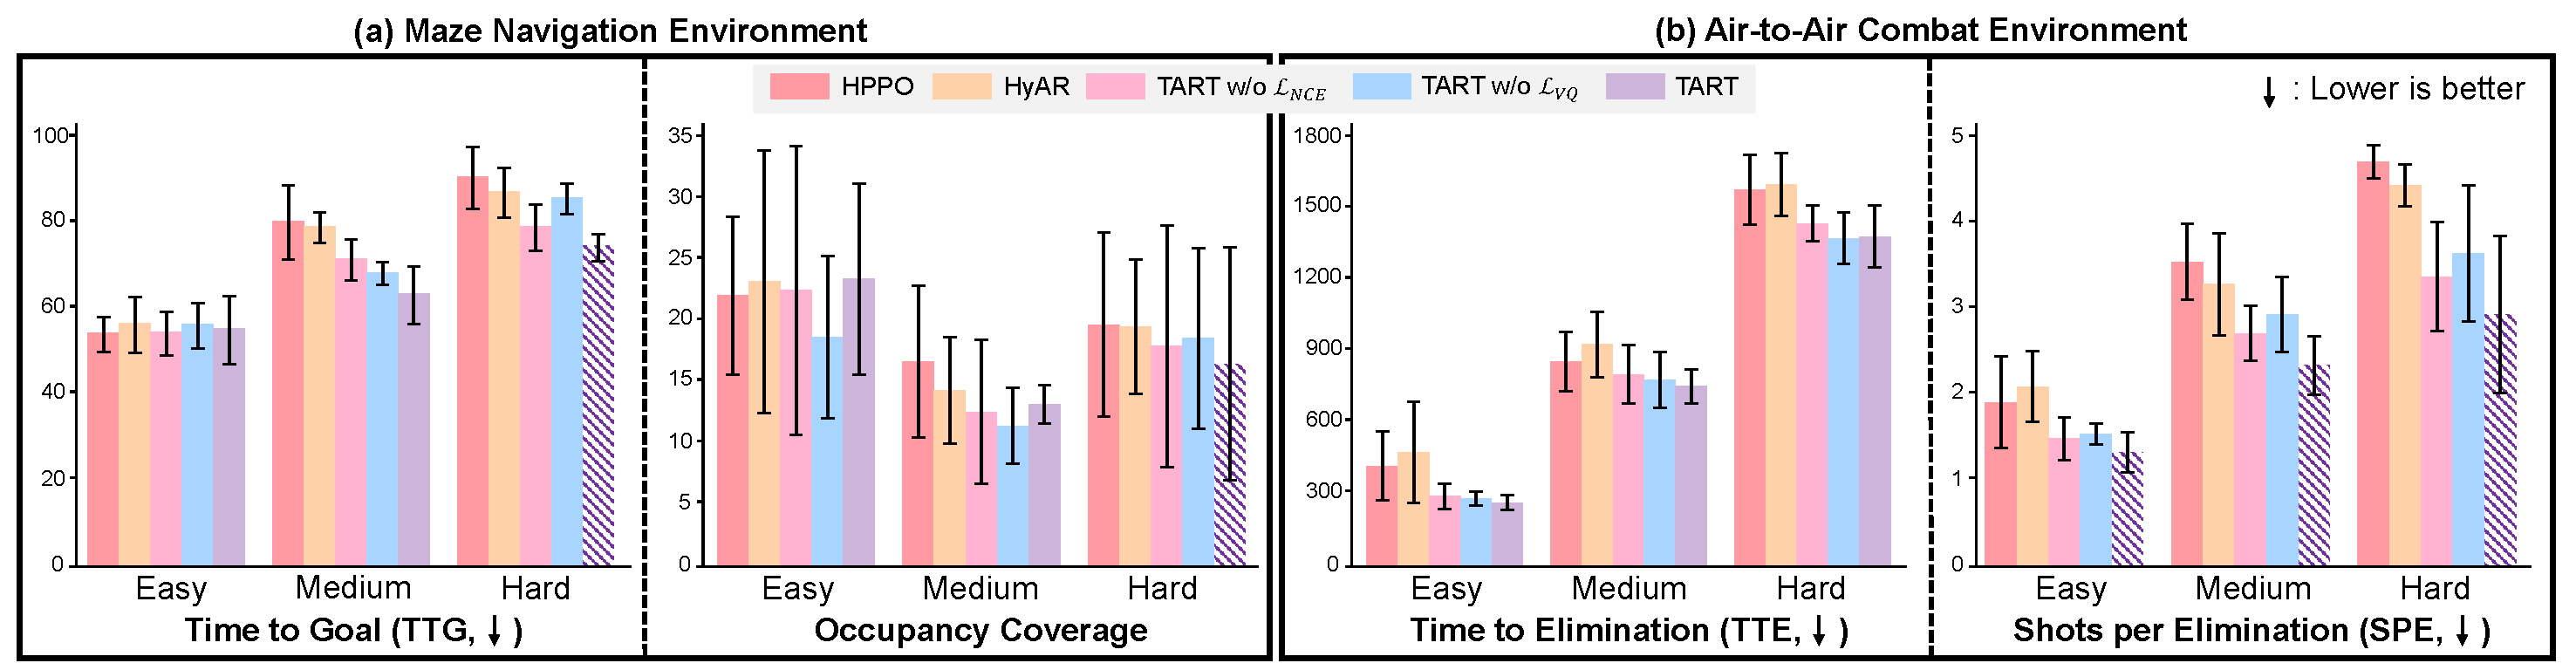
\includegraphics[width=\textwidth]{Figures/fig_4.pdf}
\vspace{-10pt}
\caption{Experimental results across the designed environments and metrics. Values are averaged over five seeds and black bars indicate standard deviation. For failed episodes, TTG and TTE are set to their maximum values (100 and 1800, respectively), while SPE is reported only for successful episodes. Hatched bars indicate the results discussed in the text and exhibiting superior performance.
}
\label{fig:quan_result}
\vspace{-10pt}
\end{figure*}

\subsubsection{Task \& Actions}
We build a high-fidelity air-to-air combat environment on top of Light Aircraft Game~\cite{liu2022light} and NeuralPlane~\cite{xue2024neuralplane}.
The platform models an F-16 aircraft with six-degree-of-freedom aerodynamics in JSBSim~\cite{berndt2004jsbsim}, equipped with short-range missiles, a gun, and defensive countermeasures.
Defensive countermeasures can neutralize an incoming missile within their effective envelope.
The objective is to eliminate the opponent before being defeated.

At each timestep $t$, the agent selects a discrete option $a_d \in \{\text{\textsc{NoOp}}, \text{\textsc{Missile}}, \text{\textsc{Gun}}, \text{\textsc{Defense}}\}$ and continuous controls $a_c \in [0, 1]^4$ corresponding to aileron, elevator, rudder and throttle.
Each episode provides a budget of five missile and five defensive countermeasures, while the gun is unrestricted but constrained by strict firing conditions~\cite{pope2022hierarchical}.
Missile launch requires a valid lock-on defined by range and aspect~\cite{liu2022light}, and is effective only if the lock persists after firing.
Gun usage follows the engagement envelope of~\cite{pope2022hierarchical}, and defensive countermeasures are effective only within a circular envelope defined as twice the missile radius.
Invalid action requests are masked without consuming the budget.
The simulator runs at 10 Hz with episodes last at most three minutes, giving a maximum horizon of $T=1800$ steps.
Episodes terminate upon opponent elimination, ownship loss (including crash), or timeout.

\subsubsection{States \& Rewards}
Following prior work~\cite{bae2023deep}, the state includes ownship kinematics (attitude, altitude, velocity, acceleration) and ego-opponent geometry (range, relative aspect), extended with remaining resources for missiles and defensive countermeasures.
The reward function consists of a sparse term for opponent elimination with dense shaping.
Tail-chase shaping~\cite{bae2023deep} rewards maintaining favorable pursuit geometry behind the opponent.
Penalties apply for being shot down or crashing at low altitude, and for each missile or countermeasure used to encourage efficiency.

\subsubsection{Scenarios \& Metrics}
We evaluate agents in three air-to-air combat scenarios (Fig.~\ref{fig:environment}(d)-(f)) of increasing difficulty, defined by opponent capability and initial geometry.
\begin{itemize}
    \item \emph{Easy}: Scripted opponent~\cite{liu2022light} with simple pursuit and evade behavior and no weapons or countermeasures. Episodes start in a pursuit geometry with the ownship behind the opponent.
    \item \emph{Medium}: Scripted opponent~\cite{liu2022light} equipped with reactive weapons and countermeasures. Episodes start in neutral geometry with opposite headings, leading to a merge after roughly one turn.
    \item \emph{Hard}: A single-agent variant of the learned pursuer~\cite{he2023autonomous} equipped with reactive weapons and countermeasures. Episodes start in neutral with an immediate merge.
\end{itemize}
Evaluation metrics are \emph{Success Rate}, \emph{Time-to-Elimination} (\textbf{TTE}) measured in decision steps with a timeout $T=1800$, and \emph{Shots-per-Elimination} (\textbf{SPE}) defined as the number of missiles required to eliminate the opponent.
\emph{Success Rate} counts episodes where the agent eliminates the opponent.
For defeats, \textbf{TTE} is set to the timeout and \textbf{SPE} to the maximum budget of five.
If an elimination occurs by gun after all missile attempts are invalidated, \textbf{SPE} is also recorded as five.

\subsubsection{Training Details}
We adopt curriculum learning~\cite{bae2023deep}, which gradually increases task difficulty to stabilize and accelerate training.
The curriculum starts with pursuit geometry and no weapons, then gradually transitions to neutral geometry while enabling weapons and defensive countermeasures.
The policy and critic follow the GRU-MLP architecture of~\cite{bae2023deep}, trained with PPO~\cite{schulman2017proximal}.
Opponents are pre-trained and remain fixed during both training and evaluation.
To ensure fairness, all baselines are trained under the same curriculum.